%\section{Appendix}
\section{Extensions}
\subsection{Set-of-Records Cleaning Model}\label{set-of-r}
In paper, we formalized the analyst-specified data cleaning as follows.
We take the sample of the records $S_{dirty}$, and apply data cleaning $C(\cdot)$.
$C$ is applied to a record and produces the clean record:
\[
S_{clean} = \{C(r) : \forall r \in S_{dirty}\}
\]
The record-by-record cleaning model is a formalization of the costs of data cleaning where each record has the same cost to clean and this cost does not change throughout the entire cleaning session.
There are, however, some cases when cleaning the first record of a certain type of corruption is expensive but all subsequent records are cheaper.

\begin{example}\label{app-ex1}
In most spell checking systems, when a misspelling is identified, the system gives an option to fix all instances of that misspelling.
\end{example}

\begin{example}\label{app-ex2}
In entity resolution problems, when an inconsistent entity is identified all other records with the same inconsistency can be efficiently fixed.
\end{example}

This model of data cleaning can fit into our framework and we formalize it as the ``Set-of-Records" model as opposed to the ``Record-by-Record" model. 
In this model, the cleaning function $C(\cdot)$ is not restricted to updating only the records in the sample.
$C(\cdot)$ takes the entire dirty sample as an argument (that is the cleaning is a function of the sample), the dirty data, and updates the entire dirty data:
\[
R'_{dirty} = C(S_{dirty},R_{dirty})
\]
we require that for every record $s \in S_{dirty}$, that record is completely cleaned after applying $C(\cdot)$, giving us $S_{clean}$.
Records outside of $S_{dirty}$ may be cleaned on a subset of dirty attributes by $C(\cdot)$.
After each iteration, we re-run the detector, and move any $r \in R'_{dirty}$ that are clean to $R_{clean}$.
Such a model allows us to capture data cleaning operations such as in Example \ref{app-ex1} and Example \ref{app-ex2}.

\subsection{Non-convex losses}\label{non-convex}
We acknowledge that there is an increasing popularity of non-convex losses in the Neural Network and Deep Learning literature. 
However, even for these losses, gradient descent techniques still apply. 
Instead of converging to a global optimum they converge to a locally optimal value. 
Likewise, \sys will converge to the closest locally optimal value to the dirty model. 
Because of this, it is harder to reason about the results.
Different initializations will lead to different local optima, and thus, introduces a complex dependence on the initialization with the dirty model.
This problem is not fundemental to \sys and any gradient technique suffers this challenge for general non-convex losses, and we hope to explore this more in the future.

\section{Proof of Lemma \ref{unbiased1}}\label{unbiased1-deriv}
\begin{lemma}
The gradient estimate $g(\theta)$ is unbiased if $g_S$ is an unbiased estimate of:
\[
\frac{1}{\mid R_{dirty} \mid} \sum g_i(\theta)
\]
\end{lemma}
\begin{proof}[Sketch]
\[
\mathbb{E}(\frac{1}{\mid R_{dirty} \mid} \sum g_i(\theta)) = \frac{1}{\mid R_{dirty} \mid} \cdot \mathbb{E}(\sum g_i(\theta)))
\]
By symmetry, 
\[
\mathbb{E}(\frac{1}{\mid R_{dirty} \mid} \sum g_i(\theta)) = g(\theta)
\]
\[
\mathbb{E}(\frac{1}{\mid R_{dirty} \mid} \sum g_i(\theta)) = \frac{\mid R_{dirty} \mid \cdot g_S + \mid R_{clean} \mid \cdot g_C  }{\mid R \mid}
\]
\end{proof}

\section{Proof of Lemma \ref{impsample}}\label{impsample-deriv}
The variance of this estimate is given by:
\[
Var(\mu) = \mathbb{E}(\mu^2)-\mathbb{E}(\mu)^2
\] 
Since the estimate is unbiased, we can replace $\mathbb{E}(\mu)$ with the average of $A$:
\[
Var(\mu) = \mathbb{E}(\mu^2)-\bar{A}^2
\]
Since $\bar{A}$ is deterministic, we can remove that term during minimization.
Furthermore, we can write $\mathbb{E}(\mu^2)$ as:
\[
\mathbb{E}(\mu^2) = \frac{1}{n^2}\sum_i^n \frac{a_i^2}{p_i}
\]
Then, we can solve the following optimization problem (removing the proportionality of $\frac{1}{n^2}$) over the set of weights $P=\{p(a_i)\}$:
\[
\min_{P} \sum_i^N \frac{a_i^2}{p_i}
\]
\[
\text{subject to: } P > 0, \sum P = 1
\]
Applying Lagrange multipliers, an equivalent unconstrained optimization problem is:
\[
\min_{P > 0,\lambda > 0} \sum_i^N \frac{a_i^2}{p_i} + \lambda \cdot (\sum P - 1)
\]
If, we take the derivatives with respect to $p_i$ and set them equal to zero:
\[
-\frac{a_i^2}{2 \cdot p_i^2} + \lambda = 0
\]
If, we take the derivative with respect to $\lambda$ and set it equal to zero:
\[
\sum P - 1
\]
Solving the system of equations, we get:
\[
p_i = \frac{\mid a_i \mid }{\sum_i \mid a_i \mid}
\]

\section{Taylor Approximation}\label{taylor-deriv}
We can take the expected value of the Taylor series expansion around the dirty value.
If $d$ is the dirty value and $c$ is the clean value, the Taylor series approximation for a function $f$ is given as follows:
\[
f(c) = f(d) + f'(d)\cdot(d-c) + ...
\]
If we ignore the higher order terms, we see that the linear term $f'(d)\cdot(d-c)$ decouples the features.
We only have to know the change in each feature to estimate the change in value.
In our case the function $f$ is the gradient $\nabla\phi$.
So, the resulting linearization is:
\[
\nabla\phi(x^{(clean)}_i,y^{(clean)}_i,\theta) \approx \nabla\phi(x,y,\theta) + \frac{\partial}{\partial X}\nabla\phi(x,y,\theta)\cdot (x - x^{(clean)}) \]
\[+ \frac{\partial}{\partial Y}\phi(x,y,\theta)\cdot (y - y^{(clean)})
\]
When we take the expected value:
\[
\mathbb{E}(\nabla\phi(x_{clean},y_{clean},\theta)) \approx \nabla\phi(x,y,\theta) + \frac{\partial}{\partial X}\nabla\phi(x,y,\theta)\cdot \mathbb{E}(\Delta x) \]
\[+ \frac{\partial}{\partial Y}\nabla\phi(x,y,\theta)\cdot \mathbb{E}(\Delta y)
\]
So the resulting estimation formula takes the following form:
\[
\approx \nabla\phi(x,y,\theta) + M_x \cdot \mathbb{E}(\Delta x) + M_y \cdot \mathbb{E}(\Delta y)
\]
Recall that we have a $d$ dimensional feature space and $l$ dimensional label space.
Then, $M_x = \frac{\partial}{\partial X}\nabla\phi$ is an $d \times d$ matrix, and $M_y = \frac{\partial}{\partial Y}\nabla\phi$ is a $d \times l$ matrix.
Both of these matrices are computed with respect to dirty data, and we will present an example.
$\Delta x$ is a $d$ dimensional vector where each component represents a change in that feature and $\Delta y$ is an $l$ dimensional vector that represents the change in each of the labels.

\section{Example $M_x$, $M_y$}\label{example-deriv}
\noindent\textbf{Linear Regression: }
\[
\nabla\phi(x,y,\theta) = (\theta^Tx - y)x
\]
For a record, $r$, suppose we have a feature vector $x$.
If we take the partial derivatives with respect to x, $M_x$ is:
\[
M_x[i,i] = 2x[i] + \sum_{i \ne j} \theta[j]x[j] - y 
\]
\[
M_x[i,j] = \theta[j]x[i]
\]
Similarly $M_y$ is:
\[
M_y[i,1] = x[i] 
\]

\vspace{0.5em}

\noindent\textbf{Logistic Regression: } 
\[
\nabla\phi(x,y,\theta) = (h(\theta^Tx) - y)x
\]
where
\[
h(z) = \frac{1}{1+e^{-z}}
\]
we can rewrite this as:
\[
h_{\theta}(x) = \frac{1}{1+e^{\theta^Tx}}
\]
\[
\nabla\phi(x,y,\theta) = (h_{\theta}(x) - y)x
\]
In component form,
\[
g = \nabla\phi(x,y,\theta)
\]
\[
g[i] = h_{\theta}(x)\cdot x[i] - yx[i]
\]
Therefore,
\[
M_x[i,i] = h_{\theta}(x)\cdot(1- h_{\theta}(x))\cdot \theta[i] x[i] + h_{\theta}(x) - y
\]
\[
M_x[i,j] = h_{\theta}(x)\cdot(1- h_{\theta}(x))\cdot \theta[j] x[i] + h_{\theta}(x)
\]
\[
M_y[i,1] = x[i] 
\]

\noindent\textbf{SVM: } 
\[
\nabla\phi(x,y,\theta) =
\begin{cases}      
-y\cdot\boldsymbol{x} \text{ if } y\cdot\boldsymbol{x}\cdot\theta \le 1 \\
0\ \text{ if } y\ \boldsymbol{x}\cdot\theta \geq 1      
\end{cases}
\]
Therefore,
\[
M_x[i,i] = \begin{cases}      
-y[i] \text{ if } y\cdot\boldsymbol{x}\cdot\theta \le 1 \\
0\ \text{ if } y\ \boldsymbol{x}\cdot\theta \geq 1      
\end{cases} 
\]
\[
M_x[i,j] = 0
\]
\[
M_y[i,1] = x[i] 
\]


\section{Experimental Comparison}
\subsection{Robust Logistic Regression}\label{rlogit}
We use the algorithm from Feng et al. for robust logistic regression.
\begin{enumerate}
\item Input: Contaminated training samples $\{(x_1, y_1), . . . ,(x_{n}
, y_{n})\}$ an upper bound on the number of outliers n, number of inliers n and sample dimension p.
\item Initialization: Set \[T = 4\sqrt{\log p/n + \log n/n}\]
\item Remove samples $(xi
, yi)$ whose magnitude satisfies $\|x_i\| \ge T$.
\item Solve regularized logistic regression problem.
\end{enumerate}

\subsection{Active Learning}\label{al}
There is a well established link between Active Learning and Online Gradient-based Algorithms \cite{guillory2009active}. 
To fairly evaluate an Active Learning methodology in these experiments, we run a gradient descent where examples are priortized by expected gradient length (explained in \cite{settles2010active}).
Ignoring the detection step, there are two differences between this algorithm and the one we propose.
First, we calculate the gradient with respect to the an estimate of the clean data, and second we sample rather than using a deterministic ordering.
While such Active Learning algorithms have been studied in the Learning Theory community, they have not been adopted in data cleaning or crowdsourcing research.
Typical algorithms include uncertainty sampling, where a classifier prioritized data closest to the margin.
However, algorithms such as uncertainty sampling focus on the narrow problem of label acquisition in hyperplane classifiers; a problem too narrow for application in this setting.

\section{Dollars For Docs Errors and Constraints}\label{dfd-errors}
The dollars for docs dataset has the following schema:
\begin{lstlisting}[mathescape,basicstyle={\scriptsize}]
Contribution(pi_speciality$\textrm{,}$ drug_name$\textrm{,}$ device_name$\textrm{,}$
corporation$\textrm{,}$ amount$\textrm{,}$ dispute$\textrm{,}$ status)
\end{lstlisting}
To flag suspect donations, we used the \texttt{status} attribute.
When the \texttt{status} was ``covered" that means it was an allowed contribution under the researcher's declared protocol.
When the \texttt{status} was ``non-covered" that means it was a disallowed contribution under the researcher's declared protocol.
The rest of the textual attributes were featurized with a bag-of-words model, and the numerical amount and dispute attributes were treated as numbers.

We cleaned the entire Dollars for Docs dataset upfront to be able to evaluate how different budgeted data cleaning strategies compare to cleaning the full data.
To clean the dataset, we loaded the entire data 240089 records into Microsoft Excel. We identified four broad classes of errors:
\vspace{0.25em}

\noindent \textbf{Corporations are inconsistently represented: } ``Pfizer", ``Pfizer Inc.", ``Pfizer Incorporated".

\vspace{0.25em}

\noindent \textbf{Drugs are inconsistently represented: } ``TAXOTERE  DOCETAXEL -PROSTATE CANCER" and ``TAXOTERE"

\vspace{0.25em}

\noindent \textbf{Label of covered and not covered are not consistent: } ``No", ``Yes",``N", ``This study is not supported", ``None", ``Combination"

\vspace{0.25em} 

\noindent \textbf{Research subject must be a drug OR a medical device and not both: } ``BIO FLU QPAN H7N9AS03 Vaccine" and ``BIO FLU QPAN H7N9AS03 Device"

\vspace{0.5em} 

To fix these errors, we sorted by each column and merged entities that looked similar and removed inconsistencies as in the status labels. 
When there were ambiguities, we refered to the drug company's website and whitepapers.
When possible, we used batch data transformations, like find and replace (i.e. the Set-of-Records model).
In all, 44234 records had some error and full data cleaning required about 2 days of efforts.

Once cleaned, in our experiment, we encoded the 4 problems as data quality constraints.
To fix the constraints, we looked up the clean value in the dataset that we cleaned up front.

\vspace{0.25em}

\noindent \textbf{Rule 1: } Matching dependency on corporation (Weighted Jaccard Similarity $>$ 0.8).

\vspace{0.25em}

\noindent \textbf{Rule 2: } Matching dependency on drug (Weighted Jaccard Similarity $>$ 0.8).

\vspace{0.25em}

\noindent \textbf{Rule 3: } Label must either be ``covered" or ``not covered".

\vspace{0.25em} 

\noindent \textbf{Rule 4: } Either drug or medical device should be null.

\vspace{0.5em}

\section{MNIST Errors}
We include visualization of the errors that we generated for the MNIST experiment.
We generated these errors in MATLAB by taking the grayscale version of the image (a $64\times 64$ matrix) and corrupting them by block removal and fuzzying.

\begin{figure}[ht]
\centering
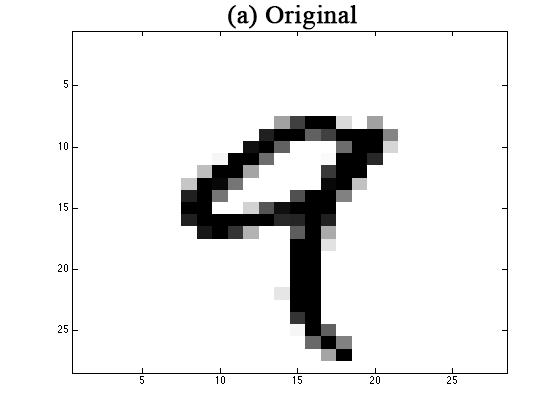
\includegraphics[scale=0.20]{exp/original.png}
 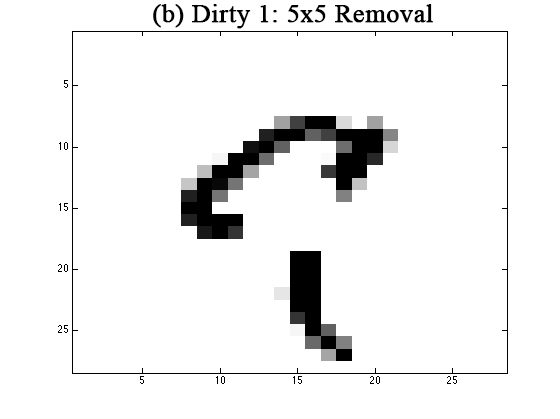
\includegraphics[scale=0.20]{exp/5x5removal.png}
 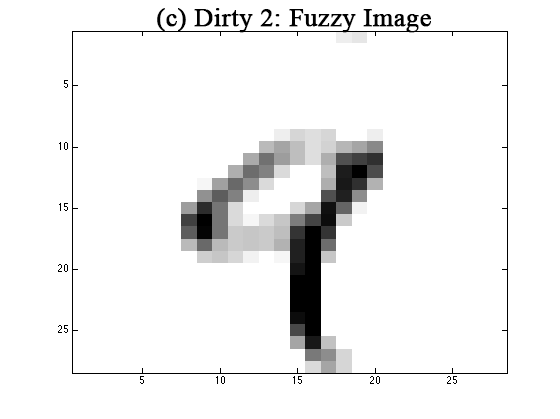
\includegraphics[scale=0.20]{exp/fuzzy.png}
 \caption{We experiment with two forms of corruption in the MNIST image datasets: 5x5 block removal and making the images fuzzy. Image (a) shows an uncorrupted ``9", image (b) shows one corrupted with block removal, and image (c) shows one that is corrupted with fuzziness. \label{mnist-corr}}
\end{figure}